\documentclass{article}
\usepackage[accepted]{icml2015}
\usepackage[utf8]{inputenc}
\usepackage{amssymb}
\usepackage{amsmath}
\usepackage{graphicx}
\usepackage{amsthm}
\usepackage{hyperref}
\usepackage{algorithm}
\usepackage{algorithmic}
\usepackage{authblk}
\usepackage{natbib}

\hyphenation{AdaBoost}

\DeclareMathOperator{\margin}{margin}
\DeclareMathOperator{\sign}{sign}
\DeclareMathOperator{\conf}{conf}
\newtheorem{definition}{Definition}
\newtheorem{theorem}{Theorem}

\begin{document}
\icmltitle{Fair Boosting: a Case Study} 

\icmlauthor{Benjamin Fish}{bfish3@uic.edu}
\icmlauthor{Jeremy Kun}{jkun2@uic.edu}
\icmlauthor{\'Ad\'am D. Lelkes}{alelke2@uic.edu}
\icmladdress{University of Illinois at Chicago \\ Department of Mathematics, Statistics, and Computer Science}

\begin{abstract} 

We study the classical AdaBoost algorithm in the context of fairness.  We use
the Census Income Dataset~\citep{UCIAdult} as a case study.  We empirically
evaluate the bias and error of four variants of AdaBoost relative to an
unmodified AdaBoost baseline, and study the trade-offs between reducing bias
and maintaining low error. We further define a new notion of fairness and
measure it for all of our methods.  Our proposed method, modifying the
hypothesis output by AdaBoost by shifting the decision boundary for the
protected group, outperforms the state of the art for the census dataset.

\end{abstract}

Although there are several papers on ``fair'' versions of learning algorithms
such as naive Bayes, decision tree learning or logistic regression, boosting,
which is one of the most successful and most widely used machine learning
algorithms, has not been studied in the context of fair learning before. In
addition to its popularity, boosting is an interesting framework in which to
study fairness because notions such as a weak learner and the boosting margin
have natural interpretations for fairness. We rigorously define these notions
in Section~\ref{sec:methods} and analyze them in Section~\ref{sec:results}.

Following previous literature, we assume that the training data is biased
against data points with a given feature value but we do not have access to the
unbiased ground truth. We want to learn a classifier which has minimal error
(as evaluated on the biased data) among all classifiers that achieve
statistical parity. \citet{DworkHPR12} point out that bias represents a notion
of group fairness rather than individual fairness, and that it is still
possible to discriminate against individuals even when achieving statistical
parity.  Thus, in addition to learning a classifier that has both low bias and
error, we want a classifier that performs well on a measure of individual
fairness.  In this paper, we introduce a notion of fairness that captures how
resistant a classifier is to bias generated independently at random against
data points wtih a given feature value.
 
The Census Income Data Set~\citep{UCIAdult} is a widely used data set for
machine learning research in which the learner's goal is to predict whether an
individual's income exceeds \$50k per year based on census data such as age,
education, gender, and marital status. In particular, when considering gender
as a protected attribute, the dataset exhibits high bias. We use this data set
as a case study to understand the fairness properties of the AdaBoost algorithm
of~\citet{FreundS97}. We provide information
about the Census data set in Section~\ref{sec:background}.

A primary advantage to using boosting is that boosting has a natural notion of
confidence which we can take advantage of to try to decrease bias while keeping
error low.  Our main empirical finding is that after boosting is performed to
produce a hypothesis $h$, flipping the output label of $h$ according to the
boosting signed confidence of the protected group outperforms the state of the art on the
Census dataset both in terms of bias and label error. We compare this to data
massaging (introduced by~\citet{KamiranC09}), replacing a standard weak learner
with a ``fair'' weak learner, and i.i.d. random relabeling. Finally, in
Section~\ref{sec:discussion} we interpret and discuss our results. 

\section{Background} \label{sec:background}

\subsection{Notions of fairness} The study of fairness in machine learning is
still young, and to the best of our knowledge we are the first to study the
fairness properties of boosting.  There are two prominent definitions of
``fairness'' that have been studied in the literature. The first is
\emph{discrimination} or \emph{bias}, which for a distribution $D$ over a set
of labeled examples $X$ with label $l : X \to \{-1, 1\}$ and a protected subset
$S \subset X$ is defined as the difference in probability of an example in $S$
having label 1 and the probability of an example in $S^C$ having label 1, i.e.
% $$ B(X, D, S) = \left | \Pr_{x \sim D|_{S^C}}[l(x) = 1] - \Pr_{x \sim D|_{S}}
% [l(x) = 1]  \right |.$$
$$ B(X, D, S) = \Pr_{x \sim D|_{S^C}}[l(x) = 1] - \Pr_{x \sim D|_{S}}
[l(x) = 1].$$
Similarly the bias of a hypothesis $h$ is the same
quantity with $h(x)$ replacing $l(x)$. If a hypothesis has low bias
in absolute value we say it achieves \emph{statistical parity.}
$S$ represents the group we wish to
protect from discrimination, and the bias represents the degree to which they
have been discriminated against.
% In this paper we will drop the absolute value
% and compute \emph{signed bias} in our charts. 
The sign of bias indicates whether $S$ or $S^C$ is discriminated against.
In particular, in this paper
bias favoring men will have positive, and bias favoring women
will have negative sign.

\citet{DworkHPR12} point out that while bias is undesirable, it does not
account for all possible forms of unfairness --- it is a measure of group
fairness rather than individual fairness.

The second notion, due to~\citet{DworkHPR12},
measures individual fairness and requires a metric on the underlying set $X$.
They call a learning algorithm ``individually fair'' if the output of the
learning algorithm is similar for individuals which are close in $X$. 

In this light, we define a new notion of fairness that departs from
previous literature in that it does not require a metric on the underlying
space. Rather, it makes the assumption that the process generating the bias is
i.i.d. random, and measures the ability for an algorithm to recover the true
labels from the biased dataset. We posit that any algorithm which is considered
``fair'' should recover from i.i.d. random bias against a protected class,
as this is a special case of more general rule-based discrimination models. We
acknowledge that this model may not accurately reflect the bias in the census
data set, but our focus is on the general fairness properties of boosting.

\subsection{AdaBoost}

Boosting algorithms work by combining \emph{base hypotheses}, ``rules of
thumb'' that are barely more accurate than random guessing, into highly
accurate predictors.  On each round, a boosting algorithm will change the
weights of the data points and find the base hypothesis that achieves the
smallest weighted error on the sample.  It always increases the weights of the
incorrectly classified examples, thus forcing the base learner to improve the
classification of the examples that are the hardest to classify correctly. In
this paper, we focus on AdaBoost, the most ubiquitous boosting algorithm. 
We omit the description of the algorithm; for an introduction to boosting
we refer the reader to \citet{SchapireF12}.
In all of our experiments we
boost decision stumps for $T=20$ rounds (after which accuracy does not
significantly improve).

% \begin{algorithm}
% \caption{AdaBoost \citep{FreundS97}}
% \begin{algorithmic}\label{adaboost}
% \FOR {$i=1$ \TO $m$}
% \STATE $D_1(i) = \frac1m$
% \ENDFOR
% \FOR {$t=1$ \TO $T$}
% \STATE $h_t = $ base hypothesis with smallest error
% \STATE $\epsilon_t = \sum_{i=1}^m D_t(i) (1-\delta_{h_t(x_i), y_i})$
% \STATE $\alpha_t = \frac12\log\frac{1-\epsilon_t}{\epsilon_t}$
% \STATE $Z_t = 2\sqrt{\epsilon_t (1-\epsilon_t)}$
% \FOR {$i=1$ \TO $m$}
% \STATE $ D_{t+1}(i) = \frac{D_t(i) e^{-h_t(x_i) y_i}}{Z_t}$
% \ENDFOR
% \ENDFOR
% \STATE $g=\sum_{t=1}^T \alpha_t h_t$
% \STATE $h = \mathrm{sgn}\circ g$
% \RETURN $h$
% \end{algorithmic}
% \end{algorithm}

Given hypotheses $h_i$ with weights $\alpha_i$ computed by AdaBoost, the
\emph{margin} of a labeled data point $(x,y)$ is
$$ \margin(x) = y\frac{\sum_i \alpha_i h_i(x)}{\sum_i \alpha_i}$$
where the $\alpha_i$'s are the weights of the base hypotheses, the $h_i$'s,
in their linear combination defined by AdaBoost.
We define the similar \emph{signed confidence} of AdaBoost for an unlabeled point $x$,
$$ \conf(x) = \frac{\sum_i \alpha_i h_i(x)}{\sum_i \alpha_i}.$$
The absolute value of the two quantities is the same, and it measures the confidence
of AdaBoost in its classification for that particular example.
The difference between the two is that whereas the sign of the margin indicates
whether the classification is correct, the sign of the confidence
tells us the classification itself. Also, the signed confidence can be computed
without access to the correct label.

It is well known that
the training error of AdaBoost decreases exponentially in the number of rounds,
and Schapire et al.~\citep{SchapireFBL98} prove that the generalization error
of AdaBoost can be bounded in terms of the empirical probability of observing a
small value of $\margin(x)$ on the training set. This
suggests that examples with small confidence are more likely to be incorrect than
examples with large margins. In particular, one might hope that one could take
advantage of this for fairness by flipping negative labels of members of the
protected class with a small confidence. Indeed, is the strategy we analyze in the
rest of this paper.

\subsection{Baseline statistics about the Census dataset}

The Census Income dataset, extracted from the 1994 Census database, contains
demographic information about $48842$ American adults.  The prediction task is
to determine whether a person earns over \$50K a year. $16192$ of the people in
the dataset are female, $32650$ are male. $30.38\%$ of men and $10.93\%$ of
women reported earnings of more than \$50K, therefore the bias of the dataset
is $19.45\%$.

We should also note that since $76\%$ of the data points have negative labels,
the constant $-1$ classifier achieves $76\%$ accuracy and perfect statistical parity.
The reader might find papers in the small fair machine learning literature
where the proposed learning algorithms have performance falling below or
barely surpassing this trivial baseline.

AdaBoost achieves an error of $15\%$ after $20$ rounds of boosting.  The bias
of the classifier output by vanilla AdaBoost is $18\%$.  We note that simply
removing the protected feature from the data does not reduce bias at all in
this case since the classifier output by vanilla AdaBoost trained for $20$
rounds on the full data doesn't explicitly use gender.

\begin{figure}[t]
\centering
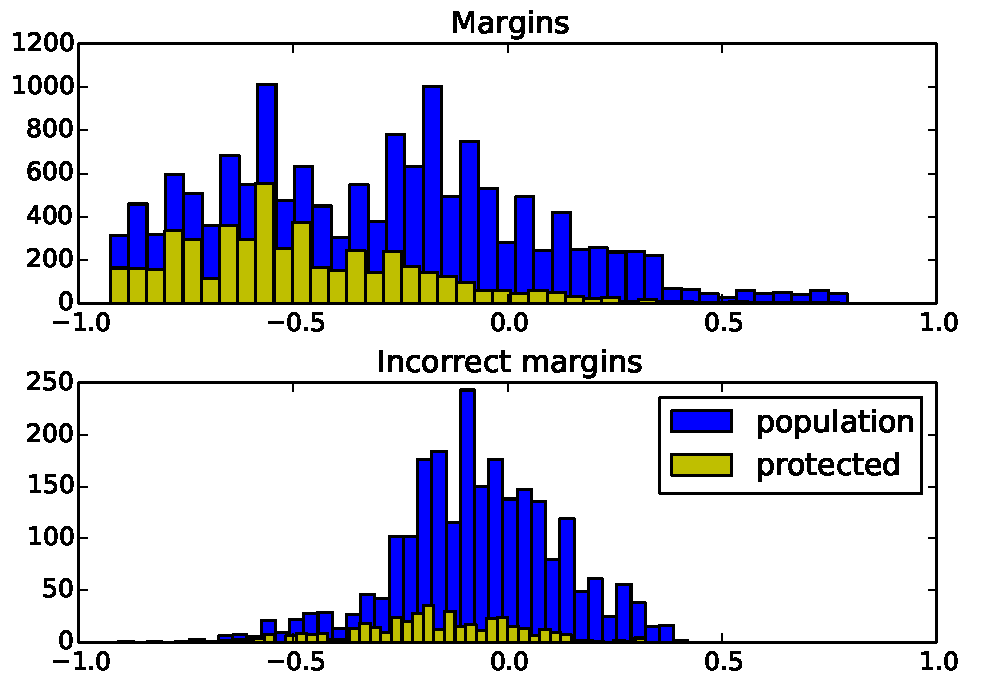
\includegraphics[width=\columnwidth]{images/censusmargins.pdf}
\caption{Histogram of boosting confidences for the Census data set. The vast
majority of women are classified as -1, and the incorrect classifications are
closer to the decision boundary.}
\label{fig:boosting-margins}
\end{figure}

\section{Methods} \label{sec:methods}

We define our methods. In what follows $X$ is a labeled dataset, $l(x)$ are the
ground truth labels, and $S \subset X$ is the protected group.  We further
assume that members of $S$ are less likely than $S^C$ to have label 1, which is
true of the Census dataset when $S$ is the women, for example.  First we
describe three relabeling algorithms.  A relabeling algorithm, when given a
hypothesis $h$ and a labeled data set $X, l$, produces a new hypothesis $h'$
that uses $h$ as a black box and flips the output of $h$ according to some
rule.

The \emph{random relabeling} (RR) algorithm computes the probability
$p$ for which, if members of $S$ with label $-1$ under $h$ are flipped by $h'$
to $+1$, the bias of $h'$ is zero in expectation.  $h'$ is then the randomized
classifier that flips members of $S$ with label $-1$ with probability $p$ and
otherwise is the same as $h$.

The \emph{shifted decision boundary} (SDB) algorithm computes the value
$\theta$ such that bias is minimized by shifting the minimum required signed
confidence for examples from $S$ from zero to $\theta$. That is, $x \in S$ then
$h'(x) = 1$ iff $\conf(x) >= \theta$, and otherwise $h'(x) = \sign(\conf(x))$
as usual. For the adult dataset $\theta < 0$.

Next, we define \emph{random massaging} (RM).  Massaging strategies, introduced
by~\citet{KamiranC09}, involve eliminating the bias of the training data by
modifying the labels of data points, and then training a classifier on this
data in the hope that the statistical parity of the training data will
generalize to the test set as well.  In our experiment, we massage the data
randomly; i.e.~we flip the labels of $S$ from $-1$ to $+1$ independently at
random to achieve statistical parity in expectation.

Finally, in \emph{fair weak learning} (FWL) we replace a standard boosting weak
learner with one which tries to minimize a linear combination of error and bias
and run the resulting boosting algorithm unchanged. The weak learner we used
computed the decision stump which minimizes the sum of label error and bias of
its induced hypothesis.

To measure fairness, we test how these algorithms are resistant to i.i.d.
random noise that introduces bias against a random subset of the individuals.
This is formalized as follows:

\begin{definition}
We define the \emph{random bias individual fairness} (RBIF) of a learning
algorithm $A$ on a labeled dataset $X,l$ as follows. Introduce a new uniformly
random binary feature $z$ on elements of $X$. Flip the labels of examples $x$
that have $z=0$ independently with probability $p$ to $-1$ to get a new dataset
$X', l'$. Run $A$ on $X', l'$ and let $h$ be the resulting hypothesis. The
random bias individual fairness of $A$ is the expected fraction of flipped
examples $x \in X'$ for which $h(x) = l(x)$.  
\end{definition}

In our experiments we set $p = 0.2$.  RBIF can be thought of as the following
experiment:  A learning algorithm is given a dataset in which bias has been
generated at random.  That is, we change the labels of a few
individuals based on a feature which is blatantly random with respect to the
classification task.  For example, we purposefully flip a few labels in the
data set of individuals who prefer chocolate ice cream over vanilla ice cream.
The goal of an algorithm is to then recover the ground truth labels in the
original dataset, recovering from the egregious bias against chocolate ice
cream lovers.  This models the ability of the algorithm to recover from bias
against a few individuals.

This definition naturally generalizes to an arbitrary distribution over
examples, but the analysis of such a definition is beyond the scope of this
short paper.

\section{Results} \label{sec:results}

In this section we state our experimental results. They are summarized in
Table~\ref{table:results}. We also included the numbers for the Learning Fair
Representations method of~\citet{ZemelWSPD13}. In that paper, the authors
implemented three other learning algorithms, these are unregularized logistic
regression, Fair Naive-Bayes \citep{KamiranC09}, and Regularized Logistic
Regression \citep{KamashimaAS11}. These methods all had errors above $20\%$;
thus we see that our confidence-based relabeling methods outperform the state of
the art.  To investigate the trade-offs made by these relabeling methods more
closely, Figure~\ref{fig:tradeoffs} shows the rate at which error increases as
bias goes to zero.

\begin{table*}
\centering
\begin{tabular}{| c | cccccc |}
\hline
               & AdaBoost & RR    & SDB  & RM   & FWL  & LFR \cite{ZemelWSPD13} \\
\hline 
label error    & 0.1529 & 0.2073 & 0.1828 & 0.1888 & 0.1820 & 0.2299 \\ 
bias           & 0.1856 &-0.0025 &-0.0036 &-0.0283 & 0.0691 & 0.0020 \\ 
RBIF           & 0.4372 & 0.4645 & 0.5340 & 0.4210 & 0.5174 & n/a \\ 
\hline 
\hline 
\end{tabular}
\caption{A summary of our experimental results for relabeling, massaging, and
the fair weak learner. The threshold for SDB was chosen to achieve perfect
statistical parity on the training data. For all methods the variance of the
results have order $10^{-4}$ or smaller, with RBIF having a slightly larger
variance than bias and label error.}
\label{table:results}
\end{table*}

\begin{figure}[t]
\centering
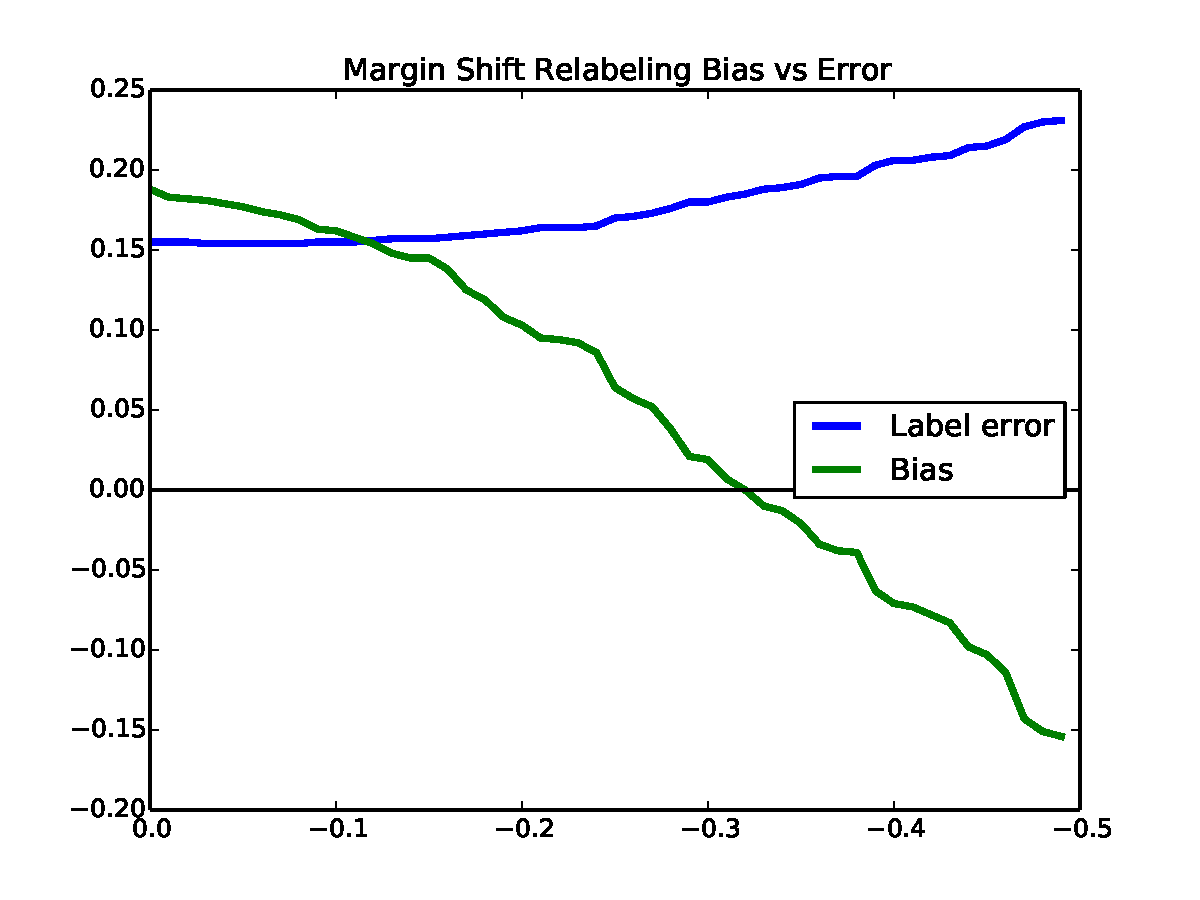
\includegraphics[width=\columnwidth]{images/relabeling-msr-tradeoffs.pdf}
\caption{Trade-off between (signed) bias and error for SDB. The
horizontal axis is the threshold used for SDB.}
\label{fig:tradeoffs}
\end{figure}

\section{Discussion}\label{sec:discussion}

Higher confidence requirement (SDB) performs equally to or outperforms every proposed
method on all measures of bias and error, including the previous state of the
art for the census dataset. Indeed, there is significant theoretical
justification that shifting the decision boundary for the protected group
achieves relatively high levels of fairness.  While it is always possible to
shift the decision boundary until statistical parity is achieved, the risk is
that some of the data points with changed labels are now labeled incorrectly,
increasing error.  For example, when the data points that are relabeled are
chosen randomly, as in RR, each is now likely to be misclassified, resulting in
an additional $5$ percent error as seen in Table~\ref{table:results}.  To
decrease error, we want to find the data points whose labels boosting was the
most unsure of since these are more likely to be classified incorrectly by
boosting.  This means we should choose the data points to relabel with the
smallest confidence, as in SDB.  Figure~\ref{fig:boosting-margins} shows that the
distribution of margins for women is noticeably shifted when compared to the
whole population, giving empirical evidence that this approach is sensible.

Of course, how data points with small confidence are relabeled does matter.  If it
is done symmetrically so that both points labeled $-1$ and $1$ are flipped,
then it takes a larger threshold to achieve statistical parity when compared to
SDB, which only flips labels from $-1$ to $1$.  This means fewer points need to
be flipped, which in turn decreases error when compared to a symmetric version.
It outperforms the baseline RR, where confidence is not considered, showing that
the points with small confidence (in absolute value) are indeed less likely to be
labeled correctly than points with large confidence.

Replacing a standard weak learner by a weak learner that tries to minimize a
combination of error and bias (FWL) does empirically reduce bias, but does not
quite achieve statistical parity. Moreover, the label error of FWL is not
better than that of SDB, and the trade-off between label error and bias cannot
easily be controlled. The same is true for random massaging (RM).

A natural baseline for RBIF is $0.5$, since a hypothesis chosen uniformly at
random will flip back half of the points that were flipped to $-1$.  Unmodified
AdaBoost encodes the bias introduced, performing worse than $0.5$.  The
question is whether we can recover from this randomly introduced bias, while
still achieving low label error and low overall bias.  Under RR, RBIF increases
marginally, as it randomly flips labels back to a label of $1$, a few of which
were the points randomly biased against.  SDB performs better than RR,
indicating that the points that were randomly biased against have small confidence
under boosting.

A further advantage of SDB is that the trade-off between label error and bias
can be controlled after training.  To decide how much bias and error we want to
allow, we do not have to fix the value of a hyperparameter before training the
algorithm, unlike for most other fair learning methods. This means that the
computational cost of choosing the best point on the trade-off curve is very
low.

While these results are preliminary, they show the advantages of fair boosting:
the confidence can be used to find a superior classifier.  We also give preliminary
results that suggest the usefulness of measuring an algorithm's resistance to
random bias.

\section*{Acknowledments}
We would like to thank Lev Reyzin for helpful discussions.

\newpage
\bibliographystyle{icml2015}
\bibliography{main}

\end{document}
\grid
